% Created 2024-07-02 mar 23:33
% Intended LaTeX compiler: pdflatex
\documentclass[presentation]{beamer}
\usepackage[utf8]{inputenc}
\usepackage[T1]{fontenc}
\usepackage{graphicx}
\usepackage{grffile}
\usepackage{longtable}
\usepackage{wrapfig}
\usepackage{rotating}
\usepackage[normalem]{ulem}
\usepackage{amsmath}
\usepackage{textcomp}
\usepackage{amssymb}
\usepackage{capt-of}
\usepackage{hyperref}
\usetheme{default}
\usecolortheme{}
\usefonttheme{}
\useinnertheme{}
\useoutertheme{}
\author{Enrique Perez, Anahi Lopez, Daniel Flores, Josue Zapata}
\date{<2024-07-2>}
\title{Corrección de Errores (E4, Q4)}

\hypersetup{
 pdfauthor={Enrique Perez, Anahi Lopez, Daniel Flores, Josue Zapata},
 pdftitle={Corrección de Errores (E4, Q4)},
 pdfkeywords={},
 pdfsubject={},
 pdfcreator={Emacs 27.1 (Org mode 9.3)}, 
 pdflang={Spanish}}
\begin{document}

\maketitle
\begin{frame}{Outline}
\tableofcontents
\end{frame}


\section{Corrección de Errores (E4, Q4)}
\label{sec:orgc883342}
\section{Introducción}
\label{sec:org9006cee}
\begin{frame}[label={sec:org685cafc}]{¿Qué es un error en memoria?}
Los errores en la memoria pueden clasificarse en dos tipos principales: errores permanentes y errores transitorios. Estos errores afectan la integridad de los datos almacenados y pueden deberse a fallas físicas o eventos aleatorios.
\end{frame}

\section{Tipos de errores}
\label{sec:org00cb5aa}
\begin{frame}[label={sec:org880c151}]{Errores permanentes}
Los fallos permanentes, también conocidos como "hard errors," son defectos físicos en la memoria que pueden deberse a problemas de fabricación o desgaste del material. Las celdas afectadas no pueden almacenar datos de manera segura.
\end{frame}

\begin{frame}[label={sec:org878cc47}]{Errores transitorios}
Los errores transitorios u ocasionales, conocidos como "soft errors," son eventos aleatorios que alteran el contenido de una o más celdas de almacenamiento sin causar daño físico permanente. Estos pueden ser causados por radiación, fluctuaciones eléctricas, o interferencias electromagnéticas.

Para garantizar la integridad de los datos almacenados en la memoria, se utilizan diversas técnicas de detección y corrección de errores. Una de las técnicas más comunes es el uso de códigos de corrección de errores, como el código de Hamming.
\end{frame}

\section{Código Hamming}
\label{sec:orgc25531d}

\begin{frame}[label={sec:org75c1411}]{Historia}
\begin{itemize}
\item En 1950, Richard W. Hamming publicó un artículo sobre detección y corrección de errores.
\item Este trabajo marcó el inicio de una nueva área en la teoría de la información.
\item Los códigos de Hamming son fundamentales en la teoría de la codificación.
\item Aplicaciones prácticas: modems, memorias, comunicaciones vía satélite.
\end{itemize}
\end{frame}

\begin{frame}[label={sec:org9f31c41}]{Usos}
\begin{itemize}
\item Detectar y corregir errores en un bit.
\item Usados en informática para asegurar la integridad de datos.
\item Se debe saber Código binario, Distancia entre dos combinaciones binarias (dada por el número de bits que hay que cambiar en una de ellas para obtener la otra), Distancia mínima de un código (es la menor de las distancias entre dos combinaciones binarias cualesquiera pertenecientes a dicho código).
\item Los códigos de Hamming son cíclicos y ponderados, utilizan puertas XOR.
\end{itemize}
\end{frame}

\begin{frame}[label={sec:orgf139804}]{Práctica}
\begin{itemize}
\item Introducción de bits de redundancia en una palabra para corrección de errores.
\item Nomenclatura: (n° bits totales, n° bits info). Ejemplo: (8, 3).
\item Bits de paridad en posiciones potencia de dos: 1, 2, 4, 8, 16\ldots{}
\item Cada bit de paridad calcula la paridad de un conjunto específico de datos.
\item Uso de tablas para representación y cálculo de paridad.
\item Posteriormente su decodificación.
\end{itemize}
\end{frame}

\begin{frame}[label={sec:orgf8a9dd1}]{Código de Hamming}
Un código corrector de errores se caracteriza por su capacidad para detectar y corregir fallas en las palabras de datos. Aunque mejora la fiabilidad de la memoria, introduce una mayor complejidad en el proceso.

El resultado de este código se llama "palabra de síndrome", la cual se busca que cumpla con las siguientes propiedades:

•Si el síndrome contiene solo ceros, no se ha detectado error.

•Si el síndrome tiene un solo bit puesto en 1, indica que se ha ocurrido un error en uno de los cuatro bits de comprobación, pero no es necesario corregirlo.

•Si el síndrome tiene más de un bit puesto en 1, el valor numérico del síndrome nos dice exactamente cuál bit de la palabra de datos corresponde corregir el error. 
\end{frame}
\begin{frame}[label={sec:orgb011659}]{Imagen Hamming}
\begin{center}
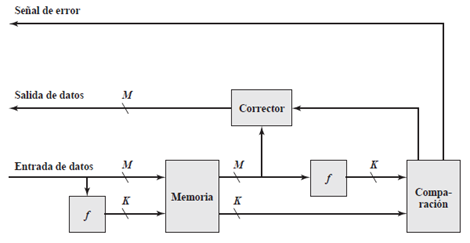
\includegraphics[width=.9\linewidth]{./imagenes/hamming.png}
\end{center}
\end{frame}

\begin{frame}[label={sec:org626836b}]{Ejemplo de código de Hamming}
Calculo de (7, 4) 7 bits, 4 bits de datos - 3 bits de paridad.

Bits de datos:  d1,d2,d3,d4

Bits de paridad: p1,p2,p3

Posiciones: p1,p2,d1,p3,d2,d3,d4

Funcionaes
p1: 1, 3, 5, 7 bit

p2: 2, 3, 6, 7 bit

p3: 4, 5, 6, 7 bit
\end{frame}

\begin{frame}[label={sec:org555a910}]{Ejemplo de código de Hamming 2}
Calculo de los bits de paridad
p1=d1( + )d2( + )d4

p2=d1( + )d3( + )d4

p3=d2( + )d3( + )d4

Ejemplo de datos:
d1 = 1, d2 = 0, d3 = 1, d4 = 1

p1= d1( + )d2( + )d4 = 1( + )0( + )1= 0

p2= d1( + )d3( + )d4 = 1( + )1( + )1= 1

p3= d2( + )d3( + )d4 = 0( + )1( + )1= 0

Cadena de bits: 0,1,1,0,0,1,1
\end{frame}

\begin{frame}[label={sec:org6e7dd0b}]{Ejemplo prueba del código}
Supongamos que durante la transmisión, el bit en la posición 5 se corrompe y se convierte en 1. Entonces, el código recibido es:
0,1,1,0,1,1,1

Para detectar y corregir el error, calculamos los bits de paridad nuevamente y los comparamos con los bits de paridad recibidos.

\begin{enumerate}
\item Recalculamos los bits de paridad:
\end{enumerate}
p'1= d1( + )d2( + )d4 = 1( + )1( + )1= 1

p'2= d1( + )d3( + )d4 = 1( + )1( + )1= 1

p'3= d2( + )d3( + )d4 = 1( + )1( + )1= 1

\begin{enumerate}
\item Comparamos los bits de paridad:
\end{enumerate}
p'1 ( + ) p1 = 1( + )0 = 1

p'2 ( + ) p2 = 1( + )1 = 0

p'3 ( + ) p3 = 1( + )0 = 1
\end{frame}
\end{document}
